%
% main.tex -- Paper zum Thema <ml>
%
% (c) 2020 Autor, OST Ostschweizer Fachhochschule
%
% !TEX root = ../../buch.tex
% !TEX encoding = UTF-8
%
\chapter{Kann ein künstliches neuronales Netzwerk die Fourier-Transformation lernen?\label{chapter:ml}}
\kopflinks{Fourier-Transformation mit Machine Learning}
\begin{refsection}
\chapterauthor{Dominik Gschwind}

%
% 0_einleitung.tex
%
% (c) 2023 Dominik Gschwind, Hochschule Rapperswil
%
% !TEX root = ../../buch.tex
% !TEX encoding = UTF-8
%
\section{Einleitung\label{ml:einleitung}}
\rhead{Einleitung}

Wir wollen untersuchen ob ein künstliches neuronales Netzwerk in der Lage ist, die Zerlegung beliebiger
Daten in Fourier-Koeffizienten zu lernen. Dazu wollen wir die algorithmische
Komplexität untersuchen und mit der schnellen Fourier-Transformation vergleichen.
\index{Komplexität, algorithmisch}%

\paragraph{Was ist ein künstliches neuronales Netzwerk?}
\emph{Künstliche neuronale
Netzwerke}\footnote{Kürzer auch nur als neuronales Netz bezeichnet mit der deutschen
Abkürzung KNN.} (englisch \emph{artificial neural networks}, ANN\footnote{In diesem Paper
\index{neuronales Netzwerk}%
\index{künstliches neuronales Netzwerk}%
wird nur die englische Abkürzung verwendet.}) werden vor allem im Gebiet der künstlichen
Intelligenz und \emph{data science} eingesetzt. Ihre Struktur und Funktionsweise ist den
biologischen neuronalen Netzwerken zum Beispiel im Gehirn nachempfunden. Prinzipiell sind
sie universelle Approximatoren\footnote{Ein Beweis dafür ist in
\cite{ml:universala-approximator-theorem} zu finden.}, das heisst sie können beliebige
Sachverhalte beliebig genau approximieren (natürlich abhängig von Struktur, Rechenaufwand,
vorhandenen Daten und weiterem).

Diese Eigenschaft ist vor allem bei künstlicher Intelligenz sehr wichtig,
da nur schon die Definition von ``Intelligenz'' noch immer ein offenes Problem in der
Philosophie ist. Andere, traditionelle Methoden wie zum Beispiel \emph{expert systems} können
\index{export system}%
nur begrenzt und mit viel Aufwand Intelligenz nachbilden.

ANNs werde aber auch vor allem dort eingesetzt, wo es keine oder nur sehr wenig erforschte
Theorie und Lösungsmethoden für eine Problemstellung gibt, oder auch Schwierigkeit und
Komplexität des Problems dessen Lösung verunmöglichen. Einige Beispiele sind
Bilderkennung, Klassifizierung, Spracherkennung oder maschinelle Übersetzung.
\index{Bilderkennung}%
\index{Klassifizierung}%
\index{Spracherkennung}%
\index{Übersetzung, maschinell}%

\medskip
In den nächsten zwei Abschnitten wollen wir diesen universellen Approximator konstruieren.
\index{Approximator}%
\index{universeller Approximator}%
Wir fangen mit einem linearen Modell an, welches uns schliesslich zum allgemein
nichtlinearen \emph{fully connected feedforward} ANN bringt.

%
% 0_lineare_regression.tex
%
% (c) 2023 Dominik Gschwind, Hochschule Rapperswil
%
% !TEX root = ../../buch.tex
% !TEX encoding = UTF-8
%

\section{Lineare Regression\label{ml:regression}}
\rhead{Lineare Regression}

\emph{Regression} ist ein statistisches Analyseverfahren mit dem Ziel, Beziehungen zwischen
Daten zu modellieren. Hat man zum Beispiel den Aktienkurs einer Firma der letzten zwanzig
Tagen, kann man mit Regression den Preis am nächsten Tag statistisch vorhersagen.
So ein Modell hat also das Ziel, die Vorhersage so gut wie möglich aus den gegebenen Daten zu approximieren.
Die einfachste Form der Regression ist die \emph{lineare Regression}, bei der alle Abhängigkeiten linear
sind.

\subsubsection{Ein lineares Modell}
\begin{itemize}
    \item $y$ soll die abhängige Variable des vorherzusagenden Wertes sein.
    \item $x_1, \cdots, x_i$ sind unabhängigen Variablen die einen Beitrag zur Vorhersage
    $y$ leisten können, genannt \emph{Features}.
    \item $\theta_0, \theta_1, \cdots, \theta_i$ sind die Koeffizienten der Features $x_i$,
    sie bestimmen wie wichtig das entsprechenden Feature ist.
\end{itemize}

Gegeben sind eine sehr grosse Anzahl $m$ Datenpunkte wobei ein Datenpunkt $j$ immer aus
den Feature-Werten $\{ x_0, x_1, \cdots, x_n \}_j$ und des vorherzusagenden Wertes $y_j$ besteht.
Am besten ist $m \gg n$. Daten die $y$-Werte enthalten, werden auch \emph{labeled data} genannt,
im Gegensatz zu \emph{unlabeled data} wo nur die Feature-Werte bekannt sind.

Man kann nun das lineare Modell mit der Gleichung
\begin{equation}
y = \theta_0 + \theta_1 x_1 + \theta_2 x_2 + \cdots + \theta_n x_n
\label{ml:regression:modell}
\end{equation}
aufstellen. Führt man die Variable $x_0 := 1$ ein, kann die Gleichung
\ref{ml:regression:modell} einfacher als
\begin{equation}
y = \sum_{i = 0}^{n} \theta_i x_i = \vec \theta \cdot \vec x =: h(\vec\theta, \vec x)
\label{ml:regression:hypothesis}
\end{equation}
geschrieben werden. Diese Beziehung wird auch \emph{hypothesis function} genannt und mit
$h$ bezeichnet.

Unser Ziel ist jetzt die Koeffizienten $\theta_i$ aus den Daten zu lernen. Hierfür
benötigen wir ein Kriterium, das uns die Distanz der Vorhersage $y_p = h(\vec x)$ zum tatsächlichen
Wert $y$ des Datenpunkts angibt. Es wird \emph{cost function} oder
\emph{loss function} genannt. Eine praktische Cost-Function ist der quadratische Fehler
\begin{equation}
J(\vec x, \vec \theta) = (y - y_p)^2.
\label{ml:regression:cost:sqerr}
\end{equation}

$J(\vec \theta)$ soll also minimiert werden, damit die Vorhersage $y_p$ möglichst nahe an den
tatsächlichen Wert $y$ kommt. Zwei allgemeine Methoden existieren, um dieses
Minimierungsproblem zu lösen.

\subsection{Minimierung mit Matrix-Inversion}

Dieses Verfahren ist auch bekannt als ``Least-Squares für überbestimmte
Gleichungssysteme''. Es verwendet die Matrix-Inversion um mit \emph{einem} Schritt an die
Lösung zu kommen.

Zuerst wird das lineare Modell aus \eqref{ml:regression:hypothesis} mit allen
$m$ Datenpunkten in Matrix-Form als
\begin{equation}
    \begin{pmatrix}
        x_{00}& \cdots& x_{0i}& \cdots& x_{0n}\\
        \vdots& \ddots& \vdots& \ddots& \vdots\\
        x_{j0}& \cdots& x_{ji}& \cdots& x_{jn}\\
        \vdots& \ddots& \vdots& \ddots& \vdots\\
        x_{m0}& \cdots& x_{mi}& \cdots& x_{mn}
    \end{pmatrix}
    \cdot
    \begin{pmatrix}
        \theta_0\\ \theta_1 \\ \vdots\\ \theta_n
    \end{pmatrix}
    = \begin{pmatrix}
        y_{0,p}\\ \vdots \\ y_{j,p} \\ \vdots \\ y_{m,p}
    \end{pmatrix}
    \quad \iff \quad
    \mathbf{X} \vec \theta = \vec y_p
    \label{ml:regression:lstsq:modell}
\end{equation}
und die Cost-Function $J$ in Matrix-Form als
\begin{align}
    J(\vec \theta) &= \sum_{j=0}^m \left(y_j - (\theta_0 x_{j0} + \theta_1 x_{j1} + \cdots + \theta_n x_{jn}) \right)^2
    = \sum_{j=0}^{m} \left( y_j - \vec \theta \cdot \vec x_j \right)^2 \nonumber\\
    &= \left(\vec y - \mathbf{X} \vec \theta\right) \cdot \left(\vec y - \mathbf{X} \vec \theta\right)
    = \left(\vec y - \mathbf{X} \vec \theta\right)^\mathrm{T} \left(\vec y - \mathbf{X} \vec \theta\right)
    \label{ml:regression:lstsq:cost}
\end{align}
formuliert. In \eqref{ml:regression:lstsq:cost} wurde die Summation über die
einzelnen quadratischen Fehler $(y_j - y_{j,p})^2$ zuerst als Skalarprodukt und
anschliessend als Matrizen-Produkt (Zeilen-Vektor mal Spalten-Vektor) geschrieben.

Um das Minimum zu finden wird der Gradient von $J(\vec \theta)$ 
\begin{align}
    \operatorname{grad} J(\vec \theta) &=
    \begin{pmatrix} \partial J / \partial \theta_0 \\ \vdots \\ \partial J / \partial \theta_n \end{pmatrix}
    = \sum_{j = 0}^{m} 2 (y_j - \vec \theta \cdot \vec x_j) \cdot
    \begin{pmatrix} - x_{j0}\\ \vdots \\ - x_{jn} \end{pmatrix} \nonumber\\
    &= \sum_{j = 0}^{m} 2 \left( \vec \theta \cdot \vec x_j - y_j \right) \cdot \vec x_j
    = \sum_{j = 0}^{m} 2 \vec \theta \cdot \vec x_j\, \vec x_j - 2 y_j \vec x_j \nonumber\\
    &= 2 \mathbf{X}^\mathrm{T} \mathbf{X}\, \vec \theta - 2 \mathbf{X}\, \vec y
    \label{ml:regression:lstsq:grad}
\end{align}
mit dem Null-Vektor $\vec 0$ gleich gesetzt
und schliesslich nach $\vec \theta$ aufgelöst:
\begin{align}
    &2\mathbf{X}^\mathrm{T} \mathbf{X}\, \vec \theta - 2 \mathbf{X}\, \vec y \overset{!}= \vec 0 \quad\Leftrightarrow\quad
    \mathbf{X}^\mathrm{T} \mathbf{X}\, \vec \theta = \mathbf{X}\, \vec y \nonumber\\
    &\implies \vec \theta = \left( \mathbf{X}^\mathrm{T} \mathbf{X} \right)^{-1} \mathbf{X} \, \vec y.
    \label{ml:regression:lstsq:formel}
\end{align}
\eqref{ml:regression:lstsq:formel} gibt eine Formel, um aus dem überbestimmten
Gleichungssystem von \eqref{ml:regression:lstsq:modell} direkt mittels Matrix-Inversion
die Koeffizienten $\vec \theta$ exakt zu berechnen.

\bigskip
Aber nicht alle solchen Matrizen sind invertierbar, sind Zeilen oder Spalten linear
abhängig oder gibt es mehr Features als Datenpunkte, kann $\mathbf{X}^\mathrm{T}\mathbf{X}$
nicht invertiert werden.
Dazu kommt dass die Matrizen-Inversion (gleich wie das Matrizen-Produkt) mit dem besten
Algorithmus, etwa $\mathcal{O}(n^{\log_2 7})$, sehr aufwendig ist.\footnote{Mehr dazu ist
in \cite{ml:computational-complexity-math-op} und
\cite{ml:computational-complexity-matrix-mult} zu finden.} Die Inversion  einer (oder
Multiplikation zweier) $1000 \times 1000$-Matrix braucht also rund $1000^{\log_2 7}
\approx 260$ Millionen Multiplikationen.

Wir haben uns hier auf die exakte Lösung der linearen Regression beschränkt mit der
simplen Cost-Function aus \eqref{ml:regression:cost:sqerr}. Später wollen wir
aber auch eine Lösung eines höchst nichtlinearen Modells mit vielleicht sehr viel
komplexerer Cost-Function berechnen können. Mit diesem Ansatz existiert aber nur
sehr selten eine Lösung in geschlossener Form (als Formel).
Mit einem geschickten Algorithmus, der die Koeffizienten $\theta_i$ numerisch
approximiert können die oben genannten Problemen weitgehend umgangen werden. Wir möchten
diesen als nächstes anschauen.

\subsection{Minimierung mit Gradient-Descent \label{ml:regression:gd}}

Betrachtet man die Cost-Function $J(\vec \theta)$ aus \eqref{ml:regression:cost:sqerr}
ergibt sich deren partielle Ableitung nach $\theta_i$ als
\begin{equation}
    \frac{\partial J}{\partial \theta_i} = 2 (\underbrace{h(\theta_0, \cdots, \theta_n, x_0, \cdots, x_n)}_{y_p} - y) \cdot x_i
    = 2 (h(\vec \theta, \vec x) - y) \cdot x_i.
\end{equation}
Es ist wieder der Gradient, ähnlich zu \eqref{ml:regression:lstsq:grad},
\begin{align}
    \operatorname{grad} J(\vec \theta)
    = 2 (h(\vec\theta, \vec x) - y) \cdot \begin{pmatrix} x_0\\ \vdots \\ x_n \end{pmatrix}
    = 2 (h(\vec\theta, \vec x) - y) \cdot \vec x.
\end{align}

Eine zentrale Eigenschaften des Gradienten ist, dass er relativ zum Auswertungspunkt immer
in die Richtung des steilsten Anstiegs zeigt. Läuft man also immer entgegengesetzt des
Gradienten und passt die $\theta_i$ entsprechend an, gelangt man nach einer gewissen
Anzahl Iterationen zu einem lokalen Minimum. Dieses Verfahren wird \emph{gradient descent}
oder deutsch \emph{Gradientenverfahren} genannt.
Konkret kann die Idee als
\begin{align}
    \vec \theta_{k+1} &= \vec \theta_{\sf k}
        - \alpha \cdot \frac{1}{2m}\sum_{j=1}^{m} \operatorname{grad} J(\vec \theta_k, \vec x_j) \nonumber\\
    &= \vec \theta_k
        - \alpha \frac{1}{m} \sum_{j=1}^{m} (h(\vec \theta_k, \vec x_j) - y_j)\cdot \vec x_j
    \label{ml:regression:gd:update}
\end{align}
geschrieben werden. Der Gradient wird als Durchschnitt über alle
Datenpunkte berechnet. Mit dem zusätzlichen Parameter $\alpha > 0$ kann die Geschwindigkeit der
Lösungsfindung eingestellt werden, er wird \emph{learning rate} genannt.

Als Startwert $\vec\theta_0$ kann beim linearen Modell irgendein Wert verwendet werden, meistens wird dieser jedoch
auf den Nullvektor $\vec 0$ gesetzt. Im Gegensatz dazu kann bei nichtlinearen Modellen der Lernvorgang
durch eine geeignete Initialisierung ernorm beschleunigt werden.

$J(\vec \theta)$ ist eine quadratische Funktion von $\theta$ mit einem einzigen lokalen
Minimum, %TODO: vielleicht Herleitung
dieses Minimum ist also auch gerade das globale Minimum. Man kann sich mit einem linearen
Modell sicher sein: Je näher der Fehler $J$ bei $0$ ist, desto näher sind die berechneten
$\theta_i$ bei den tatsächlichen $\theta_i$.

Ob oder wie schnell die Berechnung zur Lösung konvergiert ist aber von $\alpha$ abhängig.
Ein grosses $\alpha$ gibt eine schnelle Konvergenz aber auch ein grosses Potential zum
Überschiessen oder sogar zur Divergenz, bei einem kleinen $\alpha$ dauert die Lösungssuche
aber umso länger.
Für das lineare Modell \eqref{ml:regression:modell} können $\alpha$ und die Anzahl Schritte
zur exakten Lösung zum Beispiel mit dem \emph{Verfahren der konjugierten Gradienten}
einfach bestimmt werden.
Bei nichtlineare Modellen gibt es leider keine Methode um den besten Wert von
$\alpha$ zu finden. Er muss empirisch ermittelt werden, wobei am besten Werte im Bereich
$0.001$ bis $1$ auszuprobieren sind. \cite[S. 51]{ml:introduction-to-ml}


\subsubsection{Stochastischer Gradient-Descent}

Der bis jetzt beschriebene Gradient-Descent-Algorithmus berechnet einen Schritt immer über
\emph{alle} Daten, was viel Rechenleistung benötigt und schlecht parallelisiert werden
kann.
Nimmt man für jeden Berechnungsschritt eine zufällig ausgewählte, kleinere Stickprobe von
$b \ll m$ Datenpunkten, kann die Performance stark verbessert werden. $b$ wird
\emph{batch size} genannt. Die Aktualisierungsgleichung \eqref{ml:regression:gd:update} wird

\begin{equation}
  \Delta \vec\theta_{k+1} = - \alpha \frac{1}{2b} \sum_{j=1}^{b} \operatorname{grad} J(\vec
  \theta_k, \vec x_Z)
\end{equation}
mit der diskreten Zufallsvariable $Z \in \{1, 2,\cdots, m\}$.

In Fällen mit mehreren lokalen Minima kann stochastischer gegenüber dem totalen Gradient-Descent manchmal
verhindern, in diese lokalen Minima zu fallen. Je kleiner die Learning-Rate $\alpha$ gewählt
wird, desto besser wird totaler Gradient-Descent approximiert. 
\cite[S. 93ff]{ml:ml-tom-mitchell}

\subsection{Normalisierung}

Bei der Normalisierung werden alle Feature-Werte auf einen ähnlichen Bereich skaliert.
\begin{equation}
    \hat x_{ij} = \frac{2x_{ij} - (\max x_i + \min x_i)}{\max x_i - \min x_i}
\end{equation}
für ein Feature $i$ mit Datenpunkt $j$ skaliert die Feature-Werte auf den Bereich zwischen $-1$
und $1$. Es sind auch andere Methoden möglich. Dies ist vorallem dann nützlich, wenn die
einzelnen Features sehr unterschieliche Wertebereiche haben.
Die Funktionsweise wird im folgenden illustriert.

Wir haben ein Feature $a$ mit kleinem Wertebereich, zum Beispiel $a \in [0, 1]$, und ein
Feature $b \in [0, 10^6]$ mit grossem. Anfänglich hat $b$ einen viel grösseren
Effekt auf den absoluten Fehler $y - h(\vec \theta, \vec x)$ als $a$. Es muss nun
der Koeffizient von $b$ zuerst in dessen Grössenordnung gebracht werden, damit Feature $a$
überhaupt relevant wird. Wenn alle Feature-Werte in einem ähnlichen Bereich sind,
dann sind auch schon bei der ersten Iteration von Gradient-Descent alle Features relevant. Die
Kovergenz wird beschleunigt.
\section{Künstliches neuronales Netzwerk\label{ml:ann}}
\rhead{Künstliches neuronales Netzwerk}

\subsubsection{Von linearem Modell zu allgemein nichtlinearem Modell}

Im Abschnitt \ref{ml:regression} haben wird stets ein lineares Modell betrachtet.
Dem Namen ist zu entnehmen, dass es nur lineare Beziehungen abbilden kann. 
Wollen wir Abhängigkeiten höherer Ordnung oder \emph{irgendwelche} nichtlinearen
Abhängigkeiten abbilden, müssen wir dieses Modell erweitern.

Die erste Idee wäre vielleicht, das lineare Modell aus
\eqref{ml:regression:modell} viele Male hintereinander zu schalten beziehungsweise zu
verschachteln. Leider \emph{bleibt} aber eine lineare Funktion $k$-mal verschachtelt
linear.

\begin{proof}
    Es wird \eqref{ml:regression:modell} als Funktion
    \begin{equation}
        f_i(\vec x) = \vec y
        = \begin{pmatrix}
            \vec \theta_{1i} \cdot \vec x + b_{1i}\\
            \vdots\\
            \vec \theta_{ni} \cdot \vec x + b_{ni}
        \end{pmatrix}
        = \bm{\thetaup}_i \, \vec x + \vec b_i
       \label{ml:ann:linear-unit}
    \end{equation}
    genommen, wobei der konstante Anteil $\theta_0$ wieder als alleinstehender Term
    geschrieben und $b$ genannt wurde. Zudem hat $f_i(\vec x)$ gleich viele Outputs wie
    Inputs, wodurch $\vec\theta$ zu einer Matrix $\boldsymbol{\thetaup}$ und der Skalar
    $b$ zu einem Vektor $\vec b$ werden.
    
    Streng genommen ist diese Funktion nicht mehr linear im allgemeinen mathematischen
    Sinn, denn das Superpositionsprinzip gilt durch den konstanten Anteil $\vec b_i$ nicht
    mehr (im Sinne der linearen Algebra sind es affine Abbildungen und nicht lineare, die
    lineare Abbildung ist eine spezielle affine Abbildung). Der Begriff Linearität wird
    hier vielmehr im Bezug auf lineare Funktionen verwendet.

    Können wir zeigen, dass die lineare Funktion $f_i$ einmal verschachtelt wieder eine
    lineare Funktion ergibt, ist das auch für beliebig viele Verschachtelungen der Fall.
    Es wird $f_i$ einmal verschachtelt und ausmultipliziert:
    \begin{equation}
    \begin{aligned}
        \vec y_2 &= f_2(f_1(\vec x)) = (f_2 \circ f_1)(\vec x)
            = {\bm \thetaup}_2 ({\bm \thetaup}_1 \vec x + \vec b_1) + \vec b_2\\
        &= \underbrace{{\bm \thetaup}_2 {\bm \thetaup}_1}_{\tilde {\boldsymbol\thetaup}_1} \vec x
            + \underbrace{{\bm \thetaup}_2 \vec b_1 + \vec b_2}_{\tilde{\vec b}_1}
            = \tilde {\boldsymbol\thetaup}_1 \vec x + \tilde{\vec b}_1.
    \end{aligned}
    \label{ml:ann:lin-comp-proof}
    \end{equation}
    Wie \eqref{ml:ann:lin-comp-proof} zeigt ist also möglich, $f_2 \circ f_1$ wieder als lineare Funktion zu schreiben.
\end{proof}

\subsection{Aktivierungsfunktion}

Um Nichtlinearitäten einzubauen wird eine sogenannte \emph{activation function} auf
\eqref{ml:ann:linear-unit} angewendet. Die Koeffizienten-Matrix ${\bm \thetaup}$ soll
immer noch mit \hyperref[ml:regression:gd]{Gradient-Descent} gelernt werden, also muss
die gewählte Aktivierungsfunktion ableitbar bezüglich aller Inputs sein.
Eine der ersten die gebraucht wurde ist die \emph{Sigmoid}-Funktion
\begin{equation}
    \sigma(y) = \frac{1}{1+e^{-y}} \quad
    \text{mit der einfachen Ableitung}\quad
    \sigma'(y) = \sigma(y)(1- \sigma(y)).
    \label{ml:ann:activation:sigmoid}
\end{equation}
$\sigma(y)$ wird nun auf $f_i$ \emph{elementweise} angewendet, also
\begin{equation}
    g_i(\vec x) = \sigma(f_i(\vec x)) = \sigma({\bm \thetaup}_i \vec x + \vec b_i)
    = \begin{pmatrix}
        \sigma \left( \vec \theta_{1i} \cdot \vec x + b_{1i} \right)\\
        \vdots\\
        \sigma \left( \vec \theta_{ni} \cdot \vec x + b_{ni} \right)
    \end{pmatrix}.
    \label{ml:ann:one-layer}
\end{equation}

Es existieren viele weitere praktische Aktivierungsfunktionen mit guten und schlechten Eigenschaften für
eine Problemstellung, auf diese soll hier nicht weiter eingegangen werden.

\subsection{Multilayer ANN}

Für das vollständige nichtlineare Modell wird $g_i$ $k$-mal verschachtelt:
\begin{equation}
    M({\bm \thetaup}_1, \cdots, {\bm \thetaup}_n, \vec b_1, \cdots, \vec b_n) = \vec y
        = (g_1 \circ g_2 \circ \cdots \circ g_n)(\vec x) = g_n(g_{n-1}(\cdots g_1(\vec x))).
    \label{ml:ann:multilayer}
\end{equation}
So ein Modell $M$ wird \emph{fully connected \underline{f}eed\underline{f}orward
\underline{a}rtificial \underline{n}eural \underline{n}etwork}\footnote{
    Bei dieser Netzwerk-Struktur sind alle Neuronen einer Schicht mit \emph{allen} der
    nächsten Schicht vollverbunden. Volle Verbundenheit wird fast immer von der
    feedforward Struktur impliziert und wird deshalb im weiteren Text weggelassen.
} (FFANN) genannt.
Was genau bei der numerischen Berechnung passiert ist viel einfacher
in Form eines gerichteten Graphen in Abb. \ref{fig:ml:ann:simple} zu erkennen.

\begin{figure}
    \centering
    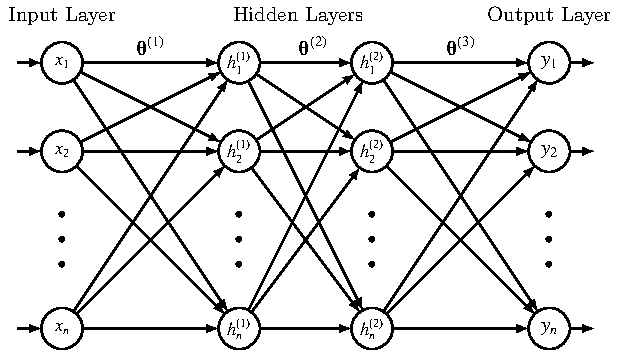
\includegraphics[scale=1]{papers/ml/images/ann_simple.pdf}
    \caption{3-schichtiges FFANN in Form eines gerichteten Graphen.}
    \label{fig:ml:ann:simple}
\end{figure}

Das Modell wird mit geschichteten Neuronen dargestellt, dabei sind bei dieser
Netzwerk-Struktur alle Neuronen einer vorherigen Schicht mit allen der nächsten verbunden.
Die Kanten zwischen den Neuronen stellen die Gewichte in der $\bm \thetaup$-Matrix
dar. Die Schichten zwischen der Eingangs- und Ausgangsschicht werden \emph{hidden layer}
genannt, da all diese Layer nicht von aussen gesehen oder angesprochen werden können.
Auf der linken Seite des Diagramms sind die Eingänge. Sie werden mit dem entsprechenden
Gewicht $\theta^{(i)}_k$ der Kante gewichtet. Anschliessend werden die gewichteten Werte
aller eingehenden Kanten plus einer Konstante $b^{(i)}_k$ summiert und darauf die
Aktivierungsfunktion der Neurone angewendet. Das Resultat ist der Eingangswert
für die nächste Schicht.
Diese Berechnung propagiert so von links nach rechts durch das Netzwerk bis am Ende die
Werte bei der Ausgangsschicht anliegen.

Die Struktur des Netzwerks, also die Anzahl Eingänge, hidden layer, Neuronen
pro Layer und Ausgänge, aber auch die spezifischen Aktivierungsfunktionen können
grundsätzlich frei gewählt werden. Sie werden \emph{hyperparameter} genannt.

\subsection{Backpropagation \label{ml:ann:backpropagation}}

Wir wollen den \hyperref[ml:regression:gd]{Gradient-Descent-Algorithmus} auch auf
unser nichtlineares Modell $M$ aus \eqref{ml:ann:multilayer} anwenden. Damit ist es aber nicht
mehr so einfach wie mit dem linearen Modell von vorher. 
$M$ besteht aus mehreren Layern, jeder mit einer Koeffizientenmatrix $\bm \thetaup$ und einem
Bias-Vektor $\vec b$. All diese Werte sollen iterativ mit Gradient-Descent gelernt werden,
sodass alle Outputs des gesamten Netzwerks möglichst nahe an den geforderten sind.

Um diese Problemstellung zu untersuchen beschränken wir uns zuerst auf den Fall eines
Netzwerks mit \emph{einem} Eingang, $n$ hidden layer mit \emph{einem} Neuron und
\emph{einem} Ausgang. Mit dieser Forderung wird die Matrizengleichung
\eqref{ml:ann:multilayer} zu einer skalaren Gleichung
\begin{equation}
    M(x, \theta_1, \cdots, \theta_n, b_1, \cdots, b_n)
    = \sigma(\theta_n \cdot \sigma( \theta_{n-1}
        \cdot \sigma ( \cdots \sigma( \theta_1 x + b_1 ) ) + b_{n-1} ) + b_n).
    \label{ml:ann:multilayer-1D}
\end{equation}

Abbildung \ref{fig:ml:ann:simple-1D} zeigt \eqref{ml:ann:multilayer-1D} wieder als
gerichteten Graphen.
\begin{figure}
    \centering
    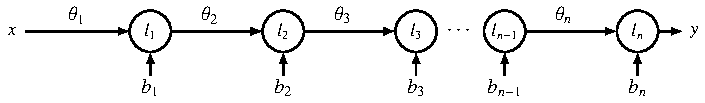
\includegraphics[scale=1]{papers/ml/images/ann_simple_1D.pdf}
    \caption{Eindimensionales FFANN.}
    \label{fig:ml:ann:simple-1D}
\end{figure}
$\theta_i$ sind die Gewichte (englisch \emph{weights}) der Verbindungen beziehungsweise
Kanten zwischen den Neuronen, $b_i$ sind die konstanten Anteile (englisch \emph{biases})
und $\sigma$ ist die Aktivierungsfunktion der Neuronen. Jedes $l_i$ soll den Output eines
Layers darstellen.

Zur weiteren Verdeutlichung wird \eqref{ml:ann:multilayer-1D} als Gleichungssystem
\begin{equation}
    \left.
    \begin{aligned}
        l_1 &= \sigma(\theta_1 x + b_1) = \sigma(\xi_1)\\
        l_2 &= \sigma(\theta_2 l_1 + b_2) = \sigma(\xi_2)\\
        &\hspace{1.5cm}\vdots\\
        y=l_n &= \sigma(\theta_n l_{n-1} + b_n) = \sigma(\xi_n)\\
    \end{aligned}
    \right\}
    \qquad\text{mit}\qquad
    \xi_i = \theta_i l_{i-1} + b_i
\end{equation}
geschrieben.

Wie schon bei Gradient-Descent im linearen Fall soll wieder die Cost-Function $J(\theta,b)
= (y - M(x, \theta, b))^2$ minimiert werden. Wir verwenden hier dieselbe Cost-Function
wie in Abschnitt \ref{ml:regression}, in der Praxis kann aber irgendeine passende und vorallem
ableitbare Funktion verwendet werden.

Es wird wieder der Gradient von $J$ gebildet, wobei die entgegengesetzte Richtung immer
noch zu einem lokalen Minimum führt. Der Gradient beinhaltet die partiellen Ableitungen
bezüglich aller Parameter

\begin{equation}
    \frac{\partial J}{\partial \theta_i} = 2(M(x) - y) \cdot \frac{\partial M}{\partial \theta_i}
    \qquad\text{und}\qquad
    \frac{\partial J}{\partial b_i} = 2(M(x) - y) \cdot \frac{\partial M}{\partial b_i}.
\end{equation}
Mit der Kettenregel
\begin{equation}
    \frac{d}{dt}f(g(t)) = \frac{df(g(t))}{d g(t)} \cdot \frac{d g(t)}{dt} = \frac{df(\tau)}{d \tau} \cdot \frac{d g(t)}{dt}
\end{equation}
lassen sich die partiellen Ableitungen von $M$ einfach berechnen.
\begin{equation}
\begin{aligned}
    \frac{\partial M}{\partial \theta_n} &= \frac{\partial l_n}{\partial \theta_n} =
    \sigma'(\theta_n l_{n-1} + b_n) l_{n-1} = \sigma'(\xi_n)l_{n-1} \\
    \frac{\partial M}{\partial \theta_{n-1}} &= \frac{\partial l_{n}}{\partial \theta_{n-1}}
    = \frac{\partial l_n}{\partial l_{n-1}} \cdot \frac{\partial
    l_{n-1}}{\partial \theta_{n-1}} = 
    \sigma'(\xi_n) \theta_n \cdot \sigma'(\xi_{n-1}) l_{n-2}
    \\
    \frac{\partial M}{\partial \theta_{n-2}} &= \frac{\partial l_{n}}{\partial \theta_{n-2}}
    = \frac{\partial l_n}{\partial l_{n-1}} \cdot \frac{\partial
    l_{n-1}}{\partial l_{n-2}}\cdot \frac{\partial l_{n-2}}{\partial \theta_{n-2}} =
    \; \sigma'(\xi_n)\theta_n \cdot \sigma'(\xi_{n-1})\theta_{n-1}\cdot \sigma'(\xi_{n-2})l_{n-3}
    \\
    \vdots\quad&\\
    \frac{\partial M}{\partial b_n} &= \frac{\partial l_n}{\partial b_n} =
    \sigma'(\xi_n) \\
    \frac{\partial M}{\partial b_{n-1}} &= \frac{\partial l_{n}}{\partial b_{n-1}}
    = \frac{\partial l_n}{\partial l_{n-1}} \cdot \frac{\partial
    l_{n-1}}{\partial b_{n-1}} = 
    \sigma'(\xi_n) \theta_n \cdot \sigma'(\xi_{n-1}) \\
    \vdots\quad&
\end{aligned}
\end{equation}

Wichtig zu erkennen ist, dass alle Werte $l_i$ sowie auch $\xi_i=\theta_i l_{i-1}+b_i$ nur
einmal berechnet werden müssen. Das Netzwerk muss sowieso für den finalen Wert $y$ einmal
ausgewertet werden, dieser Schritt wird \emph{forward propagation} (Vorwärtspropagierung)
genannt. Gleichzeitig können alle Zwischenresultate gespeichert werden, um sie für den
Korrekturschritt direkt einzusetzen.
Die Parameter werden analog zu \eqref{ml:regression:gd:update} bei jeder Iteration mit
\begin{equation}
    \theta_i \leftarrow \theta_i - \alpha \frac{\partial J}{\partial \theta_i}
    \qquad\text{und}\qquad
    b_i \leftarrow b_i - \alpha \frac{\partial J}{\partial b_i}
\end{equation}
angepasst.

Bei den partiellen Ableitungen sieht man, dass jede Schicht $i$ immer von allen
nächsten Schichten $i+1, i+2, \cdots$ mit identischer Form abhängt.
Wir wollen eine Formel herleiten, die genau den Zusammenhang von zwei
benachbarten Neuronen beschreibt. Dazu führen wir die neue Grösse 
\begin{equation}
    \delta_i = \frac{\partial J}{\partial \xi_i}
\end{equation}
ein. Sie wird auch \emph{local gradient} (lokaler Gradient) genannt. Damit können
die partiellen Ableitungen und Aktualisierungsgleichungen schon einmal vereinfacht geschrieben werden:
\begin{equation}
    \frac{\partial J}{\partial \theta_i} = \delta_i \cdot l_{i-1}
    \;\Rightarrow\; \Delta \theta_i = - \alpha \delta_i l_{i-1}
    \qquad\text{und}\qquad
    \frac{\partial J}{\partial b_i} = \delta_i
    \; \Rightarrow\; \Delta b_i = - \alpha \delta_i.
\end{equation}
Der lokale Gradient kann schliesslich mit
\begin{equation}
    \delta_{i-1} = \frac{\partial J}{\partial \xi_i} \cdot \frac{\partial \xi_i}{\partial \xi_{i-1}}
    = \delta_i \cdot \frac{\partial \xi_i}{\partial \xi_{i-1}}
    = \delta_i \cdot \sigma'(\xi_{i-1}) \theta_i
    \label{ml:ann:bp:rekursiv},
\end{equation}
wie gewünscht, rekursiv berechnet werden.

In \eqref{ml:ann:bp:rekursiv} ist noch besser zu erkennen, dass das Übertragungsverhalten
des Fehlers $\delta_{i-1}/\delta_i$
zwischen zwei Neuronen von zwei benachbarten Schichten $i$ und $i+1$ nur von der Kante
$(i)\rightarrow(i+1)$ dazwischen also dem
Gewicht, der Ableitung der Aktivierungsfunktion des Neuron in Schicht $i$ und dem lokalen
Gradienten der Schicht $i+1$ abhängt.
$\delta_n$ der letzten Schicht berechnet sich immer noch mit der partiellen Ableitung
\begin{equation}
    \delta_n = \frac{\partial J}{\partial \xi_n}
    = \frac{\partial J}{\partial M} \cdot \frac{\partial M}{\partial \xi_n}
    = 2(\underbrace{M(x)}_{l_n} - y) \cdot \sigma'(\xi_n).
\end{equation}

Die rekursive Berechnung des Fehlergradienten und somit der Anpassungsinformation für alle
Gewichte und Konstanten ist, wie wir gesehen haben, extrem simpel und performant.
Dieser Anpassungsprozess als Rückpropagierung des Fehlers wird \emph{backpropagation} genannt.

\subsubsection{Erweiterung auf allgemeine feedforward Netzwerke}

Wir haben in der Herleitung des Backpropagation-Algorithmus ein stark vereinfachtes
Netzwerk betrachtet. Mit den gleichen Überlegungen ist es aber auch möglich,
Backpropagation für ein Netzwerk mit mehreren Ein- und Ausgängen, mehreren Neuronen pro
hidden layer und verschiedenen Aktivierungsfunktionen zu machen.

Durch Summierung der Kosten aller Ausgänge kann erst einmal die Cost-Function sehr einfach
auf mehrere Outputs erweitert werden:
\begin{equation}
    \tilde J(\theta, b) = \sum_{k\in \text{Outputs}} J(M_k(x), y).
\end{equation}
Danach können die Backpropagation-Gleichungen analog aufgestellt werden:
\begin{equation}
\begin{aligned}
    \delta_{\text{node}_i}^{(\text{last layer})} &=
        \frac{\partial \tilde J}{\partial \xi_{\text{node}_i}^{(\text{last layer})}} \\
    \delta_{\text{node}_k}^{(\text{previous layer})} &=
        \sigma'_{\text{node}_k} \left( \xi_{\text{node}_k}^{(\text{previous layer})} \right) 
        \sum_{j\in \substack{\text{nodes of}\\\text{current layer}}}
        \theta_{k\rightarrow j} \cdot \delta_j\\
    \theta_{\text{node}_k\rightarrow\text{node}_j} &\leftarrow
        \theta_{\text{node}_k\rightarrow\text{node}_j} -
        \alpha \cdot \delta_{\text{node}_j} \cdot \sigma_{\text{node}_k}(\xi_{\text{node}_k}) \\
    b_{\text{node}_j} &\leftarrow b_{\text{node}_j} - \alpha \cdot \delta_{\text{node}_j}.
\end{aligned}
\label{ml:ann:bp:update}
\end{equation}

\bigskip
Unser Ziel eines universellen Approximators ist somit erreicht. In der Praxis sind die
Algorithmen für Gradient-Descent, Backpropagation und verbesserte Ableger davon in
Bibliotheken implementiert. Einige bekannte Bibliotheken für die Programmiersprache Python
sind \texttt{Keras}, \texttt{TensorFlow} und \texttt{PyTorch}.
\section{Diskrete Fouriertransformation mit ANN\label{ml:dft-with-ann}}
\rhead{DFT mit ANN}

Die \emph{diskrete Fouriertransformation} (DFT) einer Zahlenreihe $x_n \in \{ x_0, x_1, \cdots, x_{N-1}\}$
mit $N$ Elementen kann mit
\begin{equation}
    c_k = \frac{1}{N} \sum_{n=0}^{N-1} x_n e^{\normalsize -jk\frac{2\pi}{N}n}
\end{equation}
berechnet werden, oder in vektorschreibweise
    \begin{equation}
    c_k = \begin{pmatrix}
        x_0\\
        x_1\\
        \vdots\\
        x_{N-1}
    \end{pmatrix} \cdot
    \frac{1}{N} \begin{pmatrix}
        e^{-j \omega_k 0} \\
        e^{-j \omega_k 1} \\
        \vdots \\
        e^{-j \omega_k (N-1)} \\
    \end{pmatrix}
    \qquad \text{mit}\qquad \omega_k = \frac{2\pi k}{N}.
    \label{ml:dft-with-ann:dft:vector}
\end{equation}

Die einzelnen $x_n$ werden mit einem komplexen Koeffizienten gewichtet und anschliessend
summiert. In der Vektorschreibweise wird dieser Effekt mit dem Skalarprodukt erzielt. Man
erkennt, dass dies ein linearer Zusammenhang ist.

Um uns auf die reellen Zahlen zu bschränken, wird \eqref{ml:dft-with-ann:dft:vector} in
die Kosinus-Anteile $a_k = 2{\rm Re}(c_k)$ und Sinus-Anteile $b_k = -2{\rm Im}(c_k)$
unterteilt:
\begin{equation}
    a_k = \vec x \cdot \frac{2}{N} \begin{pmatrix}
        1\\
        \cos(\omega_k 1)\\
        \vdots\\
        \cos(\omega_k (N-1))
    \end{pmatrix}
    = \vec x \cdot \vec \theta_{k,a}
    \quad \text{und} \quad
    b_k = \vec x \cdot \frac{-2}{N} \begin{pmatrix}
        0\\
        \sin(\omega_k 1)\\            
        \vdots\\
        \sin(\omega_k (N-1))
    \end{pmatrix}
    = \vec x \cdot \vec \theta_{k,b}.
\end{equation}
Beide Teile sind bis auf die Koeffizienten genau gleich. Sie können  in der Form des mehrdimensionalen linearen
Modells \eqref{ml:ann:linear-unit} als
\begin{equation}
    \vec a = \begin{pmatrix}a_0\\ \vdots \\ a_{N-1} \end{pmatrix} = \begin{pmatrix}
        \vec \theta_{0,a} & \vec \theta_{1,a} & \cdots & \vec \theta_{N-1,a}
    \end{pmatrix} \vec x
    = {\bm \thetaup}_{a} \vec x
    \quad\text{und}\quad
    \vec b = {\bm \thetaup}_{b} \vec x
\end{equation}
geschrieben werden. Die konstanten Anteile entfallen.

In Abb. \ref{fig:ml:dft-with-ann:linear} ist das Netz für die Kosinus-Anteile abgebildet.
Als Übertragungsfunktion wurde für die Linearität die Identitätsfunktion $f(x) = x$ gewählt. Das Netz ist
also linear und nicht einmal affin (alle Bias-Werte sind Null). Ein analoges Netz kann
auch für die Sinus-Anteile erstellt werden. Alternativ können die Sinus-Koeffizienten aus
den Kosinus-Koeffizienten mit dem Zusammenhang
\begin{equation}
    \frac{N}{2} \arccos(\theta_{kn,a}) = \frac{N}{-2} \arcsin(\theta_{kn,b}) \quad \iff \quad
    \theta_{kn,b} = -\sin(\arccos(\theta_{kn,a}))
\end{equation}
berechnet werden.

\begin{figure}
    \centering
    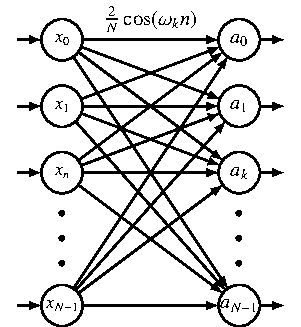
\includegraphics[scale=0.8]{papers/ml/images/ann_dft_linear.pdf}
    \caption{Lineares Netzwerk für die DFT.}
    \label{fig:ml:dft-with-ann:linear}
\end{figure}

Man kann erkennen, das so ein Netz unseren Fall der linearen Regression
(\ref{ml:regression}) exakt wiederspiegelt. Die Koeffizienten $\vec \theta_{k,a}$ und
$\vec \theta_{k,b}$ können also mit herkömmlichem Gradient-Descent gelernt werden, und das
sogar in endlich vielen Schritten, exakt.

Leider haben wir mit dieser Methodik überhaupt nichts gewonnen. Die Koeffizienten müssen
zwar nur \emph{einmal} gelernt werden bei gleichbleibendem $N$, um aber die
fouriertransformierten Werte $c_k$ zu berechnen, müssen immer noch zwei volle
Matrix-Vektor multiplikationen durchgeführt werden. Hier ist die schnelle
Fouriertransformation bei weitem überlegen.

Die Frage, ob es möglich ist mit einem künstlichen neuronalen Netzwerk die Fouriertransformation zu
berechnen können wir totzdem bejahen. Denn so ein lineares Netzwerk \emph{ist} ein FFANN,
auch wenn ein Spezialfall.

Möchte man, dass ein Modell die Fouriertransformation selber lernt, wenn es
sie benötigt, ist das mit einem nichtlinearen FFANN schlecht realisierbar und sehr
aufwändig. Ein besserer Ansatz bietet \cite{ml:pmlr-v97-dao19a}, wobei durch ein geschickt
aufgebautes lineares Netzwerk mit schwachbesetzten Schichten, Faktorisierungen von einer
vielzahl der linearen Transformationen gelernt werden können. \cite{ml:pmlr-v97-dao19a}
zeigt also, dass ein ANN mit geschicktem Aufbau in der Lage ist ein fast beliebigen
schnellen linearen Transformations-Algorithmus (zum Beispiel die FFT) aus Daten zu rekonstruieren.

\printbibliography[heading=subbibliography]
\end{refsection}
